\documentclass[11pt,a4paper]{article}

% Language setting
\usepackage[english]{babel}
\usepackage{parskip}
\usepackage{float}
\usepackage[utf8]{inputenc}
\usepackage{graphicx}
\usepackage{subcaption}
\usepackage{amsmath}
\usepackage{amssymb}
\usepackage{amsthm}
\usepackage{tikz}

\usepackage{changepage}
\usepackage{xcolor}
\usepackage{soul}
\usepackage{gensymb}
\usepackage{enumitem}
\usepackage{listings}
\lstset{
  basicstyle=\ttfamily\small,
  columns=flexible,
  breaklines=true,
  frame=single,
  xleftmargin=0.04\textwidth,
  captionpos=b
}
\usepackage[letterpaper,top=0.5in,bottom=1.0in,left=0.5in,right=0.5in,marginparwidth=0in]{geometry}

% Useful packages
\usepackage{amsmath}
\makeatletter
\newcommand{\oset}[3][0ex]{%
  \mathrel{\mathop{#3}\limits^{
    \vbox to#1{\kern-1\ex@
    \hbox{$\scriptstyle#2$}\vss}}}}
\makeatother

\usepackage[colorlinks=true, allcolors=blue]{hyperref}
\usepackage{multicol}
\graphicspath{ {Images/} }

\usepackage[utf8]{inputenc}
\usepackage{graphicx}
\usepackage{pgfplots}
\usepackage{booktabs}

\pgfplotsset{compat=1.17}

% ----------------------------
% Section / Subsection formatting
% ----------------------------
\usepackage{titlesec}
\titleformat{\section}[block]{\centering\Large\bfseries}{\thesection.}{0.5em}{}
\titleformat{\subsection}[block]{\centering\large\bfseries}{\thesubsection}{0.5em}{}

%-------------------------------------------------------------------------
\begin{document}

\break \break \break \break \break 
\begin{center}

{{\Huge Stony Brook University}}                        \break \break
{{\Huge College of Engineering \& Applied Sciences}}   \break \break
{\huge ESE 507.01: Advanced Digital System Design and Generation - Fall 2025} \break \break \break \break \break \break \break \break \break \break \break \break \break 

\end{center}

\begin{center}
    {\Huge Final Project Report} \break \break
    {\large Date: 9/27/25 - 12/12/25} \break
\end{center}
\vspace*{\fill}

\begin{center}
    {\large Ryan Lin (114737153)} \break
    {\large ryan.lin@stonybrook.edu} \break\break
    {\large \&}                   \break \break
    {\large Huabin Wu (115067644)} \break
    {\large huabin.wu@stonybrook.edu} \break
\end{center}

\newpage
\begin{center}
 {\Large Project Part 1: MAC Unit}\break   
\end{center}
\textbf{1. Use Synopsys DesignCompiler to synthesize your unpipelined design with INW=16 and OUTW=64 for a range of different clock frequencies from slow to fast. Adapt the scripts you used in HW2.\\\\
For each frequency you try, record the area, power, the critical path location, and whether the timing constraint was met or violated. In your report, make a table that shows this data for each attempted frequency. Make sure you include units on all values you report (here and everywhere else in the report). \\\\
Make graphs that show the relationships you found between clock frequency and both area and power. Explain the trends that you observed and explain why they occur. (Make two graphs. On both, show clock frequency on the x-axis; then show area as the y-axis on one graph and power as the y axis on the other.) Make sure use graphs that plot both axes proportionally (like a scatter graph, not a line graph). Only include the design points where the timing constraint is MET.\\\\
For each frequency, give a description in your report of where the critical path is. Don’t
just copy/paste the endpoints from the synthesis report, but explain logically where the
critical path lies in the module. (For example, “the critical path starts at the output of
register [register name], passes through logic that computes [description of the logic], and
ends at the input to register [register name].”)
}

\begin{figure}[h!]
    \centering
    % First plot
    \begin{subfigure}{0.48\textwidth}
        \centering
        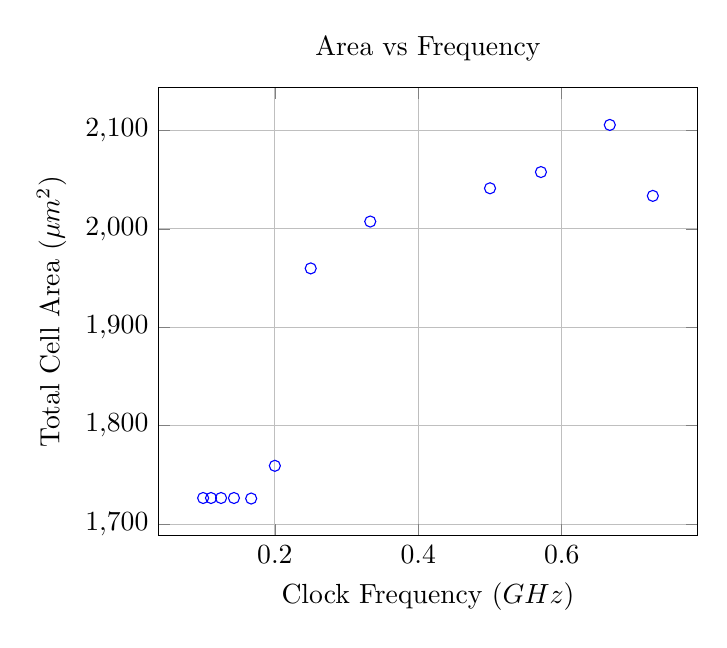
\begin{tikzpicture}
            \begin{axis}[
                xlabel={Clock Frequency ($GHz$)},
                ylabel={Total Cell Area ($\mu m^2$)},
                title={Area vs Frequency},
                grid=both
            ]
            \addplot[only marks,blue,mark=o] 
            coordinates {
                (0.727,2033.56999)
                (0.667,2105.655988)
                (0.571,2057.775989)
                (0.500,2041.283989)
                (0.333,2007.501989)
                (0.250,1959.887988)
                (0.200,1759.324001)
                (0.167,1726.07400)
                (0.143,1726.606004)
                (0.125,1726.606004)
                (0.111,1726.606004)
                (0.100, 1726.606004)
            };
            \end{axis}
        \end{tikzpicture}
    \end{subfigure}
    %\hfill
    % Second plot
    \begin{subfigure}{0.48\textwidth} 
        \centering
        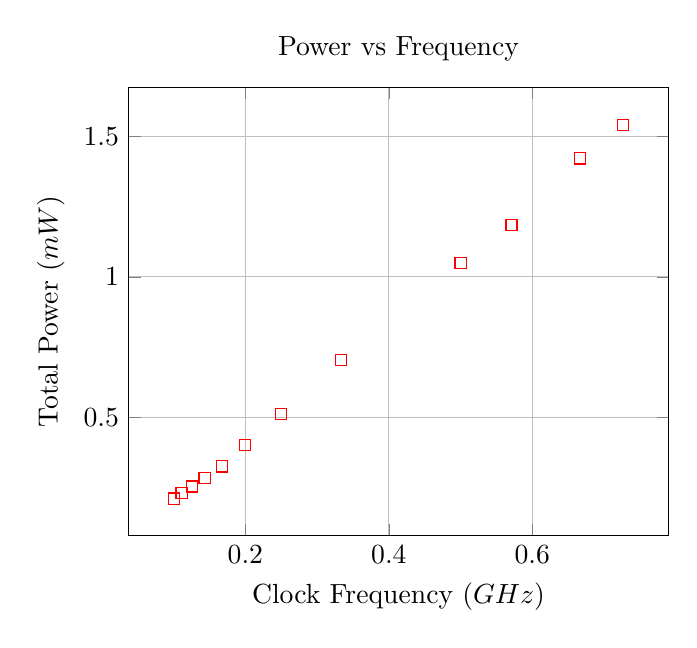
\begin{tikzpicture}
            \begin{axis}[
                xlabel={Clock Frequency ($GHz$)},
                ylabel={Total Power ($mW$)},
                title={Power vs Frequency},
                grid=both
            ]
            \addplot[only marks,red,mark=square] 
            coordinates {
                (0.727,1.4966+0.0453946)
                (0.667,1.3759+0.0466764)
                (0.571,1.1410+0.0453218)
                (0.500,1.0054+0.0446582)
                (0.333,0.6592897+0.0436944)
                (0.250,0.4698978+0.0420895)
                (0.200,0.3605876+0.0394458)
                (0.167,0.2857602+0.0384291)
                (0.143,0.2449227+0.0384279)
                (0.125,0.2143073+0.0384279)
                (0.111,0.1904954+0.0384279)
                (0.100,0.1714459+0.0384279)
            };
            \end{axis}
        \end{tikzpicture}
    \end{subfigure}
    \caption{Scatter plots of frequency vs area (left) and frequency vs power (right), only showing slack-met designs.}
\end{figure}

\begin{itemize}
    \item \textbf{Area vs Frequency:} Area increases slightly with higher clock frequencies due to the need for larger/faster cells to meet timing.
    \item \textbf{Power vs Frequency:} Power rises with frequency since dynamic power scales with $f$ while leakage stays nearly constant.
\end{itemize}

\begin{table}[h!]
\centering
\begin{tabular}{@{}cccccc@{}}
\toprule
Frequency ($GHz$)& Area ($\mu m^2$) & Total Power ($mW$)& Critical Path (Data Arrival, $ns$)& Slack Status & Slack ($ns$)\\ \midrule
0.800 & 2092.89 & 1.7235 & input0[4] $\rightarrow$ out\_reg[42] (1.29) & Violated & None \\
0.727 & 2033.57 & 1.5420 & input0[7] $\rightarrow$ out\_reg[52] (1.34) & Met & 0.0 \\
0.667 & 2105.66 & 1.4226 & input0[13] $\rightarrow$ out\_reg[41] (1.46) & Met & 0.0 \\
0.571 & 2057.78 & 1.1863 & input0[5] $\rightarrow$ out\_reg[62] (1.71) & Met & 0.01 \\
0.500 & 2041.28 & 1.0501 & input0[0] $\rightarrow$ out\_reg[63] (1.96) & Met & 0.01 \\
0.333 & 2007.50 & 0.7030 & input0[3] $\rightarrow$ out\_reg[63] (2.95) & Met & 0.02 \\
0.250 & 1959.89 & 0.5120 & input0[4] $\rightarrow$ out\_reg[63] (3.97) & Met & 0.0 \\
0.200 & 1759.32 & 0.4000 & input0[1] $\rightarrow$ out\_reg[63] (4.95) & Met & 0.0 \\
0.167 & 1726.07 & 0.3242 & input0[3] $\rightarrow$ out\_reg[63] (5.46) & Met & 0.5 \\
0.143 & 1726.61 & 0.2834 & input0[3] $\rightarrow$ out\_reg[63] (5.46) & Met & 1.5 \\
0.125 & 1726.61 & 0.2527 & input0[3] $\rightarrow$ out\_reg[63] (5.46) & Met & 2.5 \\
0.100 & 1726.61 & 0.2099 & input0[3] $\rightarrow$ out\_reg[63] (5.46) & Met & 4.5 \\ \bottomrule
\end{tabular}
\caption{MAC unpipelined design (INW=16, OUTW=64). Power is sum of dynamic and leakage. All design points shown, including slack violations.}
\end{table}





\newpage

\textbf{2. Now, repeat the tasks from question 1 for your pipelined design with the same values of INW and OUTW. Additionally, answer the following: Did pipelining help make this module faster? Explain why or why not and show how this is reflected in the synthesis data and critical path.}


\begin{figure}[h!]
    \centering
    % First plot
    \begin{subfigure}{0.48\textwidth}
        \centering
        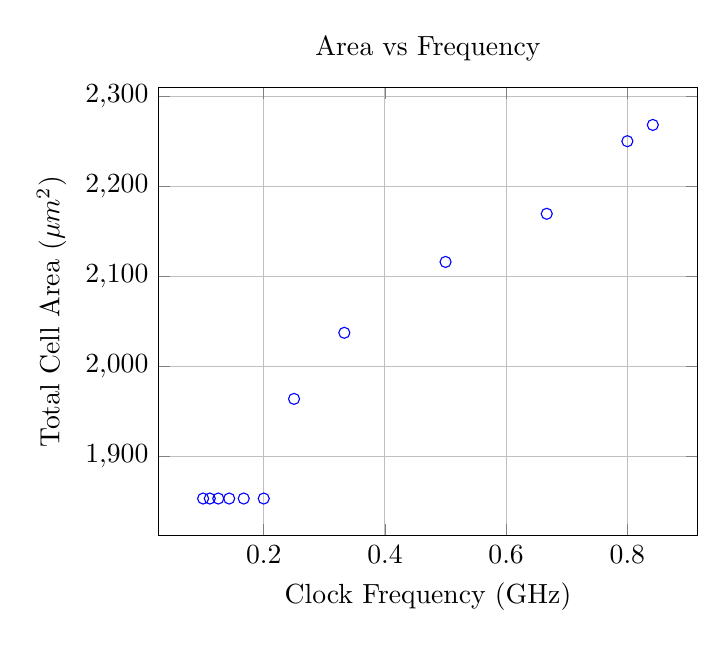
\begin{tikzpicture}
            \begin{axis}[
                xlabel={Clock Frequency (GHz)},
                ylabel={Total Cell Area ($\mu m^2$)},
                title={Area vs Frequency},
                grid=both
            ]
            \addplot[only marks,blue,mark=o] 
            coordinates {
                (0.842, 2268.181975)
                (0.800, 2250.093975)
                (0.667, 2169.495979)
                (0.500, 2116.029978)
                (0.333, 2037.293982)
                (0.250, 1963.877984)
                (0.200, 1853.22199)
                (0.167, 1853.22199)
                (0.143, 1853.22199)
                (0.125, 1853.22199)
                (0.111, 1853.22199)
                (0.100, 1853.22199)
            };
            \end{axis}
        \end{tikzpicture}
    \end{subfigure}
    % Second plot
    \begin{subfigure}{0.48\textwidth}
        \centering
        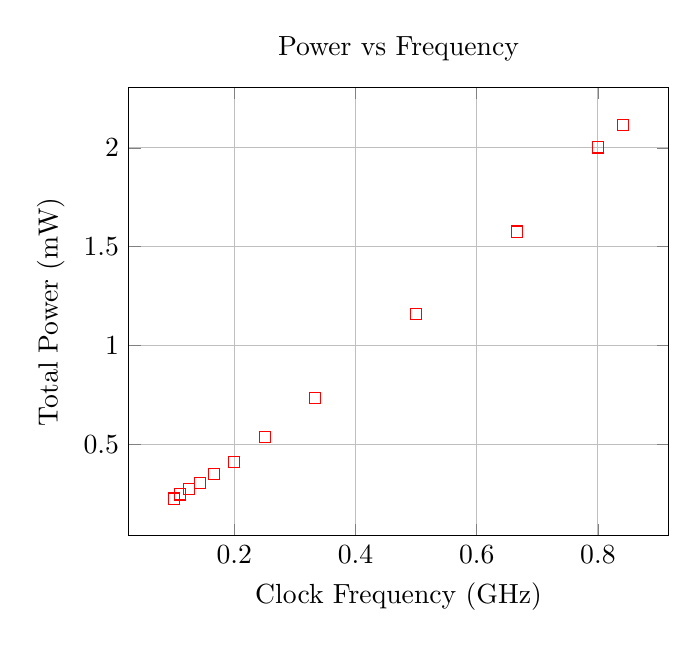
\begin{tikzpicture}
            \begin{axis}[
                xlabel={Clock Frequency (GHz)},
                ylabel={Total Power (mW)},
                title={Power vs Frequency},
                grid=both
            ]
            \addplot[only marks,red,mark=square] 
            coordinates {
                (0.842,2.0649+0.0506906)
                (0.800,1.9517+0.0501332)
                (0.667,1.5286+0.0476742)
                (0.500,1.1115+0.0458313)
                (0.333,0.6903037+0.0453784)
                (0.250,0.4946457+0.0431071)
                (0.200,0.3728040+0.039699)
                (0.167,0.3106700+0.039699)
                (0.143,0.2664936+0.0396796)
                (0.125,0.2331819+0.0396796)
                (0.111,0.2072728+0.0396796)
                (0.100,0.1865455+0.0396796)  
            };
            \end{axis}
        \end{tikzpicture}
    \end{subfigure}
    \caption{Scatter plots of frequency vs area (left) and frequency vs power (right), only showing slack-met designs.}
    \label{piped_plot}
\end{figure}

\begin{itemize}
    \item \textbf{Area vs Frequency:} Area increases slightly with higher clock frequencies due to the need for larger/faster cells to meet timing.
    \item \textbf{Power vs Frequency:} Power rises with frequency since dynamic power scales with $f$ while leakage stays nearly constant.
\end{itemize}

\begin{table}[h!]
\centering
\resizebox{\textwidth}{!}{
\begin{tabular}{@{}cccccc@{}}
\toprule
Frequency (GHz) & Area ($\mu m^2$) & Total Power (mW) & Critical Path (Data Arrival, ns) & Slack Status & Slack (ns) \\ \midrule
1.000 & 2298.77 & 2.5754 & input0[4] $\rightarrow$ piped\_product\_reg[21] (1.13) & Violated & None \\
0.889 & 2328.03 & 2.3171 & input0[13] $\rightarrow$ piped\_product\_reg[28] (1.14) & Violated & None \\ 
0.842 & 2268.18 & 2.1156 & input0[8] $\rightarrow$ piped\_product\_reg[20] (1.16) & Met & 0.0 \\
0.800 & 2250.09 & 2.0018 & input0[1] $\rightarrow$ piped\_product\_reg[24] (1.22) & Met & 0.0 \\
0.667 & 2169.50 & 2.0053 & input0[7] $\rightarrow$ piped\_product\_reg[30] (1.46) & Met & 1.46 \\
0.500 & 2116.03 & 1.1573 & piped\_product\_reg[31] $\rightarrow$ out\_reg[63] (1.96) & Met & 0.0 \\
0.333 & 2037.29 & 0.7357 & input0[2] $\rightarrow$ piped\_product\_reg[30] (2.96) & Met & 0.0 \\
0.250 & 1963.88 & 0.5378 & out\_reg[0] $\rightarrow$ out\_reg[63] (3.95) & Met & 0.01 \\
0.200 & 1853.22 & 0.4125 & out\_reg[0] $\rightarrow$ out\_reg[63] (4.87) & Met & 0.1 \\
0.167 & 1853.22 & 0.3504 & out\_reg[0] $\rightarrow$ out\_reg[63] (4.87) & Met & 1.1 \\
0.143 & 1853.22 & 0.3062 & out\_reg[0] $\rightarrow$ out\_reg[63] (4.87) & Met & 2.1 \\
0.125 & 1853.22 & 0.2729 & out\_reg[0] $\rightarrow$ out\_reg[63] (4.87) & Met & 3.1 \\
0.111 & 1853.22 & 0.2470 & out\_reg[0] $\rightarrow$ out\_reg[63] (4.87) & Met & 4.1 \\
0.100 & 1853.22 & 0.2262 & out\_reg[0] $\rightarrow$ out\_reg[63] (4.87) & Met & 5.1 \\
\bottomrule
\end{tabular}
}
\caption{MAC pipelined design (INW=16, OUTW=64). Power is sum of dynamic and leakage. All design points shown, including slack violations.}
\end{table}


\break
\textbf{3. For the pipelined design with the maximum clock frequency you found, how much energy
would your system consume if it were to process a sequence of 50 sets of input values? Assume you have to wait until the final output comes out of the system, and don’t forget that your pipelined design takes more than 50 cycles to compute 50 sets of inputs.\\
Remember: energy is measured in joules. Power = energy per time. 1 Watt = 1 Joule / 1
second. Use the power obtained from synthesis and your understanding of the time it would
take for your system to fully compute 50 sets of input values.}

If we have 50 sets of inputs, then it would take 51 clock cycles to completely process all 50 sets of inputs. This is because our pipelined design is now separated into two stages where two different sets of inputs can be processed at the same time (one per stage) per clock cycle. The maximum clock frequency our pipelined design can handle without violating slack is 0.842 GHz. The total power, which includes the total dynamic power and cell leakage power, used is 2.1156mW.
Thus, the total energy consumed for 50 sets of inputs would be
\[
(107.8956\,\text{mW}) \times 51 \times (1.1875\,\text{ns}) = 6.5344\,\text{nJ}.
\]\\
\textbf{4. Would the energy you computed in question 3 change if you resynthesized the design targeting different clock frequencies? Explain and justify your answer. Think carefully about what changes when you change the target frequency and how those changes affect the power the system consumes.}

If the target clock frequency changes in synthesis, then the power consumption would alter alongside it. There is a direct relationship between clock frequency and total power consumed for our synthesized design, as seen in Figure~\ref{piped_plot}.\\\\

\textbf{5. Make a table that compares the power, area, latency, and throughput of your pipelined and unpipelined MAC designs (at the maximum clock frequency you previously found) with INW=16 and OUTW=64. In your report show how you calculated the latency and throughput. Quantify latency in seconds (or ns), and quantify throughput in terms of MACs per second. (If needed, review these concepts in the Topic 6 slides.) Based on the trade-offs seen in your table, explain when it would make sense for a designer to choose the pipelined design and when it would make sense to use the unpipelined design.}

\begin{table}[H]
\centering
\caption{Comparison of Unpipelined and Pipelined MAC Designs (INW=16, OUTW=64)}
\label{tab:mac_comparison}
\begin{tabular}{|c|c|c|c|c|c|}
\hline
\textbf{Design} & \textbf{Max Freq ($GHz$)}& \textbf{Power ($mW$)}& \textbf{Area ($\mu m^2$)} & \textbf{Latency ($ns$)}& \textbf{Throughput ($MACs/sec$)}\\ \hline
Unpipelined & 0.727 & 1.5420 & 2033.57 & 1.375 & $7.27\times10^{8}$ \\ \hline
Pipelined & 0.842 & 2.1156 & 2268.18 & 2.375 & $1.684\times10^{9}$ \\ \hline
\end{tabular}

\vspace{0.5em}
\begin{minipage}{0.95\linewidth}
\vspace{0.5em}
\textbf{Note:}
\begin{itemize}
    \item[-] Latency is the minimum clock period required for one stage — in this case, it's the time delay from the multiply register to the accumulate register.
    \item[-] Latency~(ns) $= 1.375 \times 1$ stage \quad (for unpipelined design)
    \item[-] Latency~(ns) $= 1.1875 \times 2$ stages $= 2.375$ \quad (for pipelined design)
    \item[-] Throughput~(MACs/s) $= 1\ \text{MAC per cycle} \times 0.727\ \text{GHz} = 727\ \text{million MACs/s}$
    \item[-] Throughput~(MACs/s) $= 1\ \text{proper MAC per cycle *across two stages assuming steady state*} \times 0.842\ \text{GHz} = 842\ \text{million MACs/s}$
    \item[-] We considered MACs to be operations performed per stage; so either a multiply operation or an accumulate operation can count as a MAC.
\end{itemize}
    \vspace{0.5em}
    Based on the results of the table, a designer would choose an unpipelined design if he/she wish for lower latency, and choose a pipelined design if he/she wish for higher throughput. The tradeoff is between the latency (to get a multiply-added output from a set of inputs) and the throughput (in operations and inputs per second).
\end{minipage}
\end{table}

\textbf{6. Your design is pipelined as much as possible if you assume that you cannot pipeline the arithmetic units themselves. However, as we discussed in Topic 6, we could also pipeline the multiplier itself. For example, you can replace the multiplier with one that is pipelined into more stages. Based on your results to questions 1 and 2, would you expect that deeper pipelining in the multiplier might help you reach higher clock frequencies? Justify why or why not.\\\\
If you were to pipeline the multiplier in this way, what other changes would you have to make in your module?\\\\
Would pipelining the adder be possible and a good idea? Why or why not?\\\\
(Answer this question based on your understanding of the design and your answers to prior questions. You do not need to modify your design/code to answer this question.)}\\

The multiplier of the design can be pipelined by segmenting our set of inputs (input0 and input1) into smaller streams that could be stored in registers and multiplied concurrently. For example, if INW $=$ 16, then the two inputs (input0 and input1 [15:0]) can be separated into eight groups of two-bit [1:0] values that are multiplied simultaneously. Doing so may result in a possible higher target clock frequency for our system because smaller bit-length value multiplication operations can be performed per piped stage, thus less combinational logic may be required for data to travel from one register to another. However, we are still limited by the critical path from the accumulator register's output back to its adder. \\

Pipelining the adder is also possible and beneficial in this design. Since adders typically involve carry propagation across multiple bits in the combinational path, in our case, across the OUTW bit width, it is a good idea to partition the accumulator adder's inputs into smaller bit segments. By inserting pipeline registers between these segments, the addition can be performed over multiple stages. Similar to pipelining the multiplier, it allows simultaneous processing of smaller sum segments and effectively reduces the critical path delay, improving the overall clock frequency.\\\\

\textbf{7. In questions 1 and 2, you always synthesized using the same parameter values of INW=16 and OUTW=64. Here, explore how changing INW and OUTW affects the critical path location and maximum clock frequency of your pipelined MAC module. Don’t forget: to change these parameters for synthesis, you should edit the default parameter values in your source code (mac\_pipe.sv).\\\\
First, do a set of experiments where you set INW=12 and synthesize three designs with OUTW=24, 48, and 64.\\\\
Next, do a new set of experiments where you set OUTW=48 and synthesize three designs with INW=8, 16, 24.\\\\
Do the clock frequency and critical path location change as OUTW changes? Do they change when INW changes? Explain what you see and what you learn from it. You should expect to see differences in the scaling behavior of INW and OUTW. Explain why they behave differently.\\\\
Include the six synthesis reports for this question along with your Final Report.\\}

The minimum clock frequency and the path of the critical path are as follows:

\begin{table}[h!]
\centering
\caption{Synthesis results for different (INW, OUTW) configurations (pipelined MAC)}
\label{tab:inw-outw-results}
\begin{tabular}{@{}ccc@{}}
\toprule
Parameter Config. & Minimum Clock Period ($ns$)& Crit. Path (Startpoint $\rightarrow$ Endpoint)\\ \midrule
INW=12, OUTW=24 & 1.0555  & \texttt{input0[3]} $\rightarrow$ \texttt{piped\_product\_reg[19]} \\
INW=12, OUTW=48 & 1.0670  & \texttt{input0[11]} $\rightarrow$ \texttt{piped\_product\_reg[23]} \\
INW=12, OUTW=64 & 1.0535  & \texttt{input0[5]} $\rightarrow$  \texttt{piped\_product\_reg[19]} \\[0.5em]
INW=8,  OUTW=48 & 0.8430  & \texttt{input0[3]} $\rightarrow$ \texttt{piped\_product\_reg[10]} \\
INW=16, OUTW=48 & 1.2800  & \texttt{input0[6]} $\rightarrow$ \texttt{piped\_product\_reg[30]} \\
INW=24, OUTW=48 & 1.4850  & \texttt{input0[21]} $\rightarrow$ \texttt{piped\_product\_reg[34]} \\
\bottomrule
\end{tabular}
\end{table}

\noindent Observations and explanation:
\begin{itemize}
    \item[-] The maximum frequency is related to the bit width of the input parameter \texttt{INW}, but not so much to the bit width of the output parameter \texttt{OUTW}. We can observe that the minimum clock period per synthesized design increases as the bit width of the input \texttt{INW} increases. There were minimal changes in the minimum clock period when \texttt{INW} stays constant while \texttt{OUTW} increases.
    
    \item[-] At a higher level, the location of the critical path does not change significantly. It starts from either set of the inputs and ends at the piped product register, \texttt{piped\_product\_reg}. However, when we zoom in, the critical path location changes slightly. The specific order of the bit element of each bit array changes for both the input and \texttt{piped\_product\_reg}. This is because, on the lower-level abstraction, each bit in the input and output arrays maps to different gate-level networks, which may result in slight variations in propagation delay.\\\\
\end{itemize}


\textbf{8. The MAC’s accumulator holds OUTW bits. As you know, if the value stored in the accumulator grows large enough, it will overflow. That is, OUTW bits may not be enough to store the resulting number.\\\\
Assume INW~=~5 and OUTW~=~16. What is the maximum number of MACs your system could
perform while guaranteeing that the accumulator cannot overflow? (Hint: what is the
largest magnitude number you could produce on the multiplier’s output? Then, how many
accumulations would it take for that number to produce an overflow in the accumulator?)
Don’t forget that our values are all signed integers, and don’t forget that the accumulator can be initialized to a signed INW-bit number. Show your reasoning and justify your answer.}


Given:
\[
\mathrm{INW}=5 \quad\Rightarrow\quad \text{each input}\in[-2^{4},\,2^{4}-1]=[-16,\,15],
\]
so the largest magnitude possible from a single multiply (two signed INW-bit values) is
\[
\max|\text{product}| = 16 \times 16 = 256.
\]

The accumulator is \(\mathrm{OUTW}=16\) bits, so its signed range is
\[
\text{accumulator} \in [-2^{15},\,2^{15}-1] = [-32768,\,32767].
\]

To guarantee no overflow when repeatedly accumulating the worst-case magnitude product (all products have the same sign and magnitude 256), we must consider the worst initialization of the accumulator (the initialization that gives the smallest headroom in the direction of accumulation). For positive-direction accumulation the worst initial accumulator value is \(+15\) (the largest INW signed initialization). Thus require
\[
-16 + 256\cdot N \le -32768,
\]
where \(N\) is the number of MAC accumulations. Solving:
\[
256\cdot N \le -32768 + 16 = -32752,
\]
\[
N \le \left\lfloor \frac{32752}{256} \right\rfloor = \left\lfloor 127.96875 \right\rfloor = 127.
\]

(Checking the negative direction gives the same integer bound: starting at \(-16\) and repeatedly adding \(-256\) would underflow at the same count \(N=127\).)

\bigskip
\noindent\textbf{Answer:} The maximum number of MAC accumulations that can be performed while \emph{guaranteeing} the 16-bit accumulator will not overflow (for \(\mathrm{INW}=5,\;\mathrm{OUTW}=16\)) is
\[
\boxed{N_{\max} = 127.}
\]\\


\textbf{9. If you worked with a partner, please carefully describe each partner’s contribution to this
part of the project. (If you did not work with a partner, skip this.)}

Huabin: Wrote the unpiped and piped MAC modules, simulated and synthesized both designs with different input and output bit width parameters. Answered conceptual questions and performed required calculations for the lab report.

Ryan: Wrote a python script program to parse the data of interest (area, total power consumption, critical path, slack time) from the synthesized file to speed up the process of collecting data points for tables and graphs. Assisted in formatting the lab report.

\newpage
\begin{center}
 {\Large Project Part 2: Output FIFO}\break   
\end{center}

\textbf{1. The basic form of the FIFO was discussed in class, but here you needed to adapt that to interface its output with AXI-Stream. Explain how you did that and how your logic works. }

When it comes to designing a FIFO AXI-stream system, we need to think and view it from the perspective of being in between the input interface of one module and the output interface of another module. In this part of the project, we made several adjustments to accommodate for this. Firstly, we have control signals such as TVALID and TREADY from both interfaces telling us when a module is ready to transmit and or receive data. When the FIFO is not empty, that means it can have valid data coming out of it (OUT\_TVALID). When the FIFO is not full, that means it is ready to receive data (IN\_TREADY). Notice that both these control signals are actually two different modules interfacing with each other, hence creating an extra layer of security, namely the AXI-stream handshake, that respects the FIFO flow. 

\textbf{2. Previously you synthesized this design with OUTW=24 and DEPTH=19. In your report, give the maximum clock frequency and the area, power, and critical path location for this frequency. Note that the critical path location may be somewhat confusing. Make sure you carefully trace it so you can thoroughly explain what logic the critical path includes. (Don’t just list the critical path’s start and end points; explain what the logic is doing between them.)}

\begin{table}[h!]
\centering
\caption{Synthesis results of different (OUTW, DEPTH) configurations for Output FIFO}
\label{tab:inw-outw-results}
\resizebox{\textwidth}{!}{
\begin{tabular}{@{}ccccc@{}} % <-- Changed from ccc to ccccc (5 columns now)
\toprule
Parameter Config. & Area ($\mu m^2$) & Power ($mW$) & Max. Freq. ($GHz$) & Crit. Path (Startpoint $\rightarrow$ Endpoint)\\ \midrule
OUTW=12, DEPTH=19 & 1907.48597 & 1.3436 & 1.13636  & \texttt{input0[3]} $\rightarrow$ \texttt{piped\_product\_reg[19]} \\
OUTW=24, DEPTH=19 & 3711.76393 & 2.3152 & 1.05263  & \texttt{input0[11]} $\rightarrow$ \texttt{piped\_product\_reg[23]} \\
OUTW=24, DEPTH=38 & 6798.95990 & 5.1237 & 1.07526  & \texttt{input0[5]} $\rightarrow$  \texttt{piped\_product\_reg[19]} \\
\bottomrule
\end{tabular}
}
\end{table}

\textbf{3. Repeat question 2 with both:\newline
a. OUTW=12 and DEPTH=19\newline
b. OUTW=24 and DEPTH=38\newline
Report all statistics for both designs. Explain the trends you see in area, power, and frequency. In other words, explain how these three sets of parameters affect the area, power, and frequency, and explain why.}

We see a clear trend in higher area and power consumptions as the absolute values of the OUTW and DEPTH parameters increase. More importantly, the OUTW parameter has a significant impact. This is intuitive because wider memory words will result in more congested routing and larger multiplexing logic to select from wider bit-length word data. This  obviously requires more power and spacing to be processed. 

However, we notice an odd trend observing the maximum frequency. Higher DEPTH actually resulted in a slightly short minimum clock period yield given that the OUTW parameter remains unchanged. 

The critical path from read\_ptr register to data\_out register likely goes into address decoders and multiplexers selecting from memory array blocks and through data\_out registers. This makes sense as we can see from the SystemVerilog code statement “data\_out $\leftarrow$ mem[read\_addr];”.

The critical path from capacity register to data\_out register likely stems from capacity comparison logic, and it likely goes into OUT\_AXIS\_TVALID control signal that routes to read enable signal, and out the data\_out register.

The changes in critical path and the slight decrease in maximum frequency is likely due to the way our synthesis tool handles the memory architecture used to hold word data. From (12,19) $\rightarrow$ (24,19), the critical path changes because our OUT\_AXIS\_TVALID signal after capacity comparison contains higher fanouts. From (24,19) $\rightarrow$ (24,38), pre-existing optimized memory tools might handle the delays better than the design created from our code.

\newpage
\begin{center}
 {\Large Project Part 3: Input Memory Module}\break   
\end{center}

\textbf{1. This part of the project required you to design a significant amount of control logic that interacts with the AXI-Stream interface, the memories, the K and B registers, and the inputs\_loaded and compute\_finished signals. Carefully and thoroughly document this module including your control logic. Your documentation should allow the reader to fully understand how your input\_mems module works (and any submodules) without looking at the code.}

The inputs\_mem module is a memory block that holds key important components necessary for computing a convolution operation. The module include registers that contain the following information:

\begin{itemize}
    \item A weight 'W' matrix for which its dimensions are defined by KxK, where the value of K is read and stored in a MAXK-bit register during the first cycle of every weight matrix read.
    \item An optional bias 'B' value that is stored in an INW-bit register on the cycle following the completion of the weight matrix read.
    \item An input 'X' matrix for which the kernel matrix is performing the convolution operation on.
\end{itemize}

In our system, the control flow of our inputs\_mem module is implemented via a finite state machine with five states: idle\_state, input\_W\_matrix\_state, input\_B\_value\_state, input\_X\_matrix\_state, and inputs\_loaded\_state. 

We begin in the idle\_state where we wait for any valid inputs to be picked up via AXI-stream input interface. At this point, we look for the control bit "new\_W" sent during the same cycle to be "set". If it is, then we know to transition from the idle\_state to the input\_W\_matrix\_state and that there is a new input weight matrix to consider. However, if "new\_W" was not "set", then we transition to the input\_X\_matrix\_state, and keep the weight matrix and bias value from the most recent loaded inputs to compute the next convolution against. However, we must have a weight matrix inside our memory register, and a bias value inside our 'B' register before any input 'X' matrix can be read afterwards.

There are two different complete flows:
% \begin{enumerate}[label=\alph*.]
%     \item idle\_state $\Rightarrow$ input\_W\_matrix\_state $\Rightarrow$ input\_B\_value\_state $\Rightarrow$ input\_X\_matrix\_state $\Rightarrow$ inputs\_loaded\_state $\Rightarrow$ idle\_state
%     \item idle\_state $\Rightarrow$ input\_X\_matrix\_state $\Rightarrow$ inputs\_loaded\_state $\Rightarrow$ idle\_state
% \end{enumerate}
\usetikzlibrary{automata, positioning, arrows}
\begin{figure}[H]
    \centering
    \begin{tikzpicture}[->, >=stealth, shorten >=1pt, auto, node distance=2.8cm,
                        semithick, state/.style={circle, draw, minimum size=1.5cm, align=center}]

        % State Nodes
        \node[state, initial] (idle) {Idle};
        \node[state] (W) [above right=of idle] {Input W\\Matrix};
        \node[state] (B) [right=of W] {Input B\\Value};
        \node[state] (X) [below right=of idle] {Input X\\Matrix};
        \node[state] (loaded) [below left=of X] {Inputs\\Loaded};

        % Transitions for Flow (a): New Weight Matrix
        \path (idle) edge [bend left] node {new\_W==1} (W)
              (W)    edge             node {} (B)
              (B)    edge [bend left] node {} (X);

        % Transitions for Flow (b): Reuse Weights
        \path (idle) edge [bend right] node [swap] {new\_W==0} (X);

        % Shared Transitions
        \path (X)      edge             node {} (loaded)
              (loaded) edge [bend left] node {compute\_finished==1} (idle);

    \end{tikzpicture}
    \caption{Finite State Machine flow for Inputs Memory Module}
    \label{fig:fsm_diagram}
\end{figure}

It is important to know that the inputs\_mem module can be both written to and read from depending on what state logic we are at. At the inputs\_loaded\_state, the writing freezes by "setting" the "inputs\_loaded" control signal and we let the AXI-stream's output interface handle all of the necessary reading and computation before "setting" the "compute\_finished" control signal, telling us to go back to idle\_state and watch for the "new\_W" control bit.

\vspace{1em}

\textbf{2. The number of cycles required by this module is largely determined by: the parameters (R, C), the value of K for this input, and how the testbench asserts AXIS TVALID. However, there are places where you as the designer could make choices that affect the number of cycles required by your module. For example, if your system unnecessarily sets AXIS TREADY to 0, or it adds extra cycles of delay between steps, the system will be less efficient. One way to quantify this is to measure how long your system takes to complete a task. Run a simulation where you set INW=10, R=15, C=13, MAXK=7 and INPUT VALID PROB=1. When new\_W == 1, the testbench will begin by feeding in the $K*K$ values of w, then the value of B, then the $R*C=15*13=195$ values of x. In other tests where new\_W == 0, the system will simply feed in the $R*C=15*13=195$ values of x. Simulate this design in Questa Sim's waveform view and count the number of cycles between when your design sets AXIS TREADY to 1, and when it sets inputs\_loaded to 1. Do this for a few sets of inputs where new\_W == 1 and a few sets of inputs where new\_W == 0, and record the number of cycles and the value of K. Hint: you can view the amount of simulated time that passes in the waveform and then divide it by 10ns to get the number of simulated clock cycles. In your report, for each test give this cycle count and the value of K (for both new w of 0 and 1). In the report, quantify how efficient your system is with respect to the number of clock cycles by computing the following ratios:
\begin{itemize}
    \item When new\_W == 1, use efficiency = ($K*K+1+R*C$)/cycles
    \item When new\_W == 0, use efficiency = $R*C$/cycles
\end{itemize}
In these metrics, 1.0 is perfectly efficient a good implementation will be close to this. Report both metrics and the data you collected. If your efficiency number is not close to 1, where could your logic be improved?}

The following table:

\begin{table}[h!]
\centering
\begin{tabular}{@{}cccc@{}}
\toprule
\textbf{new\_W} & \textbf{K} & \textbf{\# of cycles} & \textbf{Efficiency} \\ \midrule
1 & 3 & 205 & 1 \\ 
1 & 7 & 245 & 1 \\ 
1 & 4 & 212 & 1 \\ 
0 & X & 195 & 1 \\ 
0 & X & 195 & 1 \\ 
0 & X & 195 & 1 \\ \bottomrule
\end{tabular}
\end{table}

\vspace{1em}

\textbf{3. In the previous question, you measured the cycle count. Now, use your understanding of your system's behavior to write equations for the cycle count with respect to R, C, and K. You should have one equation for new W == 1, and one equation for new W == 0.}

The cycle count equations are defined as:
\[
\text{\# cycles} = 
\begin{cases} 
K^2 + R \cdot C + 1 & \text{if } \texttt{new\_W} = 1 \\
R \cdot C & \text{if } \texttt{new\_W} = 0 
\end{cases}
\]

\vspace{1em}

\textbf{4. For the Part 3 submission (above), you synthesized the design with parameters:
\begin{itemize}
    \item INW = 24, R = 9, C = 8, MAXK = 4
    \item INW = 10, R = 15, C = 13, MAXK = 7
\end{itemize}
For each set of parameters, report the clock frequency, area, power, and critical path location. Carefully explain each design's critical path. Don't just list its start and end points; explain what logic is included in the path and what it means. Does the critical path location change between these two designs? Explain why or why not.}

The following table:
\begin{table}[h!]
\centering
\resizebox{\textwidth}{!}{%
\begin{tabular}{@{}llllp{6cm}@{}}
\toprule
Parameter Config. & Area ($\mu m^2$) & Power ($mW$) & Max Freq. ($GHz$) & Crit. Path (Startpoint $\rightarrow$ Endpoint)\\ \midrule
INW=24, R=9, C=8, MAXK=4 & 16581.38 & 16.57 & 1.342 & \texttt{current\_state\_reg[2]} $\rightarrow$ \texttt{X\_memory\_inst/data\_out\_reg[13]} \\ 
INW=10, R=15, C=13, MAXK=7 & 18666.82 & 19.37 & 1.198 & \texttt{current\_state\_reg[2]} $\rightarrow$ \texttt{X\_memory\_inst/data\_out\_reg[4]} \\ \bottomrule
\end{tabular}%
}
\end{table}

\newpage
\begin{center}
 {\Large Project Part 4: Top-Level 2D Convolution System}\break   
\end{center}

\textbf{1. This part of the project required you to design a significant amount of control logic that interacts with the existing modules. Carefully and thoroughly document how your top-level system works, especially your control logic. Your documentation should allow the reader to fully understand how it works without looking at the code.}

The top level convolution module that connects all of the other modules, that is, \texttt{mac\_pipe} module, \texttt{fifo\_out} module, and \texttt{inputs\_mem} module, utilizes a significant amount of control signal logic together with a finite state machine to handle the control flow of the overall system. The finite state machine has six states:

\begin{itemize}
    \item \texttt{IDLE\_STATE}
    \item \texttt{INIT\_PIXEL\_STATE}
    \item \texttt{COMPUTING\_ACC\_STATE}
    \item \texttt{WRITE\_PIXEL\_STATE}
    \item \texttt{WRITE\_FIRST\_ADDR}
    \item \texttt{DONE\_STATE}
\end{itemize}

The most important control signals are:
\begin{itemize}
    \item \texttt{COMPUTE\_FINISHED\_DATA\_IN}
    \item \texttt{DATA\_AVAILABLE}
    \item \texttt{MAC\_OUTPUT\_VALID}
    \item \texttt{INITIALIZE\_ACCUMULATOR}
\end{itemize}

The complete flows are as follows:
\begin{figure}[H]
    \centering
    \begin{tikzpicture}[->, >=stealth, shorten >=1pt, auto, node distance=4.0cm,
                        semithick, state/.style={circle, draw, minimum size=1.6cm, align=center, font=\small}]

        % Node Placement: 
        % Top Row: Idle -> Init -> Compute
        % Bottom Row: Done <- Wait <- Write
        
        \node[state, initial] (idle) {Idle};
        \node[state] (init) [right=of idle] {Init\\Pixel};
        \node[state] (comp) [right=of init] {Comput.\\Acc};
        
        \node[state] (write) [below=of comp] {Write\\Pixel};
        \node[state] (wait) [below=of init] {Wait\\First\\Addr};
        \node[state] (done) [below=of idle] {Done};

        % Transitions
        
        % Idle -> Init
        % Added line break and align=center to fit text
        \path (idle) edge node[align=center] {\texttt{inputs\_loaded}\\==1} (init);
        
        % Init -> Compute
        \path (init) edge node {} (comp);
        
        % Compute -> Write
        \path (comp) edge node {} (write);
        
        % Write -> Wait (Loop Back)
        % Added line break to prevent overlap
        \path (write) edge node [swap, align=center] {next output\\pixel} (wait);
        
        % Wait -> Init (Close Loop)
        \path (wait) edge node {} (init);
        
        % Write -> Done (Exit Loop)
        \path (write) edge [bend left=25] node[align=center] {all $(R-1)(C-1)$\\written} (done);
        
        % Done -> Idle
        \path (done) edge (idle);

    \end{tikzpicture}
    \caption{Finite State Machine flow for Top-Level 2D Convolution System}
    \label{fig:top_level_fsm}
\end{figure}

In the IDLE\_STATE, the system will wait for valid data to flow in via the AXI-stream input interface. All control signals are "off" in this state. The system transitions out of the IDLE\_STATE into the INIT\_PIXEL\_STATE when the kernel weight matrix and the input 'X' matrix along with the kernel size and the bias value are all properly loaded into the inputs\_mem registers.

During the INIT\_PIXEL\_STATE, we initialize a singular pixel of the resulting 'Y' matrix (R\_out, C\_out) with the bias value for one cycle. This bias value is then added to the result of the matrix multiplication, specific to the pixel we are computing (R, C). In this state, we also keep track of the position of the input matrix that we are performing the matrix multiplication on, and reset the pointers of the kernel matrix position back to the beginning ($i=0, j=0$).

Following the INIT\_PIXEL\_STATE is the COMPUTING\_ACC\_STATE, which is where the matrix multiplication actually happens for ideally, $K^2$ number of cycles handled by the mac\_pipe module.

Once the COMPUTING\_ACC\_STATE finishes, it will transition to the WRITE\_PIXEL\_STATE where the control signal "MAC\_OUTPUT\_VALID" is "set" and the corresponding output 'Y' pixel gets written to the buffer in the fifo\_out module. In this state, we increment our cursor to the next starting pixel in the output 'X' matrix and continue the matrix multiplication for the next output 'Y' pixel.

When we finish writing the entire output 'Y' matrix to the fifo\_out module, the system transitions to the DONE\_STATE where the control signal "COMPUTE\_FINISHED\_DATA\_IN" is set and the system gets ready to load in the next input 'X' matrix or it can load in a new set of matrices (including both 'X' and weight matrix) along with a new bias value while "idling" in the IDLE\_STATE.

\vspace{1em}

\textbf{2. In Part 3, you wrote equations that described the number of cycles that the input\_mems module requires (given R, C, and K) when new\_W == 0 and new\_W == 1. Now, you should use your understanding of your system to write equations to describe the number of cycles for the entire convolution operation in the same scenarios. Your equations should reflect the best-case number of cycles between when your system starts receiving inputs and when it is done with that computation and ready to receive a new set of inputs (where "best case" implies that INPUT\_TVALID and OUTPUT\_TREADY are always 1). Don't forget that you can do simulations to verify your equations. Based on your equations, is your system's performance limited by any one phase of execution? For example, if your input loading time is much higher than the compute time, this shows that the input loading time limits your speed much more than computation. On the other hand, if the system spends most of its time doing MAC operations on data, then the computational unit is the limiting factor. If the times are close to balanced, then this shows your system's performance is highly dependent on both of them. Importantly, keep in mind that this answer can change based on the values of R, C, and K. In other words, you may find you are limited by one factor when they are small, and another when they are large. Think carefully and explain fully. Justify and explain your answers.}

For parameters $R=9$, $C=8$, $K=5$:

\textbf{Case 1: \texttt{new\_W} = 1}
\begin{equation*}
\begin{split}
\text{Cycles} &= \underbrace{(RC + 1 + K^2 + 1)}_{\text{Initial Load}} \\
&\quad + \underbrace{[((R-K+1)(C-K+1)) - 1]}_{\text{Pixels } 1 \dots (N-1)} \times \underbrace{(1 + (K^2 + 1) + 1 + 1)}_{\text{Latency per Pixel}} \\
&\quad + \underbrace{(1 + (K^2 + 1) + 1 + 1)}_{\text{Last Pixel (set compute finished)}} \\
&= 99 + (19 \times 29) + 29 \\
&= \mathbf{679 \text{ cycles}}
\end{split}
\end{equation*}

\textbf{Case 2: \texttt{new\_W} = 0}
\begin{equation*}
\begin{split}
\text{Cycles} &= \underbrace{(RC + 1)}_{\text{Initial Load}} \\
&\quad + \underbrace{[((R-K+1)(C-K+1)) - 1]}_{\text{Pixels } 1 \dots (N-1)} \times \underbrace{(1 + (K^2 + 1) + 1 + 1)}_{\text{Latency per Pixel}} \\
&\quad + \underbrace{(1 + (K^2 + 1) + 1 + 1)}_{\text{Last Pixel}} \\
&= 73 + (19 \times 29) + 29 \\
&= \mathbf{653 \text{ cycles}}
\end{split}
\end{equation*}

The system spends the majority of the time loading inputs in the inputs\_mem module during the IDLE\_STATE and the multiply-accumulate operations state. This is dictated by how large the parameters R, C, and K are. If $R*C \gg K*K$ then the system spends most of its time computing the MAC operation. On the other hand, if $K*K \approx R*C$, then the system spends approximately a balanced amount of time between doing the input loading and the MAC operation. Of course, this also depends on if new\_W is "set" or not. If new\_W is not "set", then loading the inputs during the IDLE\_STATE will take "$K*K + 1$" less number of cycles as compared to if it was set because we aren't loading in any new kernel weight matrix and bias values, but just solely loading a new input 'X' matrix instead.

\vspace{1em}

\textbf{3. For the Part 4 submission, you synthesized the design with three sets of parameters:
\begin{itemize}
    \item INW = 12, R = 9, C = 8, MAXK = 5
    \item INW = 18, R = 9, C = 8, MAXK = 5
    \item INW = 24, R = 16, C = 17, MAXK = 9
\end{itemize}
For each set of parameters, report the maximum clock frequency, minimum clock period, area, and power. For each, describe where the critical path is in the design. (Make sure you explain the critical path fully; don't just list the start and end points.) If the different designs have meaningfully different critical path locations, explain or speculate as to why the location changes. You only need to report data for the smallest clock period you were able to find for each design.}

\begin{table}[h!]
\centering
\resizebox{\textwidth}{!}{%
\begin{tabular}{@{}llllp{6cm}@{}}
\toprule
Parameter Config. & Area ($\mu m^2$) & Power ($mW$) & Max Freq. ($GHz$) & Crit. Path (Startpoint $\rightarrow$ Endpoint)\\ \midrule
INW=12, R=9, C=8, MAXK=5 & 21703.74 & 17.78 & 0.90497 & \texttt{input\_mems\_instantiation/ X\_memory\_inst/data\_out\_reg[5]} $\rightarrow$ \texttt{mac\_pipe\_instantiation/ piped\_product\_reg[22]} \\ 
INW=18, R=9, C=8, MAXK=5 & 31465.41 & 20.58 & 0.72463 & \texttt{input\_mems\_instantiation/ X\_memory\_inst/data\_out\_reg[5]} $\rightarrow$ \texttt{mac\_pipe\_instantiation/ piped\_product\_reg[34]} \\ 
INW=24, R=16, C=17, MAXK=9 & 164809.08 & 97.02 & 0.63291 & \texttt{input\_mems\_instantiation/ X\_memory\_inst/data\_out\_reg[20]} $\rightarrow$ \texttt{mac\_pipe\_instantiation/ piped\_product\_reg[41]} \\ \bottomrule
\end{tabular}%
}
\end{table}

\vspace{1em}

\textbf{4. Now, find the throughput of the second and third of the three designs you considered in question 3:
\begin{itemize}
    \item INW = 18, R = 9, C = 8, MAXK = 5
    \item INW = 24, R = 16, C = 17, MAXK = 9
\end{itemize}
(All of the following questions will refer to these two designs.) Find the throughput of each of the two designs under three different assumptions about testbench parameters INPUT\_TVALID\_PROB and OUTPUT\_TREADY\_PROB: 0.1, 0.5, and 1. (That is, do three simulations for each design, one where both \_PROB parameters are 0.1, one where they are both 0.5, and one where they are both 1.) For each, record the number of clock cycles needed for 10,000 convolutions, as reported by the testbench with the parameters set appropriately. Then use those cycle counts along with the clock periods you found from synthesis to find the throughput in number of convolutions per second for each design under the three assumptions of the\_PROB parameters. In your report, make a table that shows the cycle counts and computed throughputs for all 6 scenarios (two designs with three sets of assumptions each). Make sure your tables include units (here and in all questions).}

The following table:

\begin{table}[h!]
\centering
\resizebox{\textwidth}{!}{%
\begin{tabular}{|c|c|c|c|c|}
\hline
\textbf{} & \multicolumn{2}{c|}{\textbf{Design 1}} & \multicolumn{2}{c|}{\textbf{Design 2}} \\
\textbf{} & \multicolumn{2}{c|}{(INW=18, R=9, C=8, MAXK=5)} & \multicolumn{2}{c|}{(INW=24, R=16, C=17, MAXK=9)} \\ \hline
\textbf{TVALID/TREADY prob.} & \textbf{Cycle Count} & \textbf{Throughput ($ops/sec$)} & \textbf{Cycle Count} & \textbf{Throughput ($ops/sec$)} \\ \hline
0.1 & 13400388 & 540758 & 74805492 & 84607 \\ \hline
0.5 & 7017694 & 1032586 & 51462470 & 122985 \\ \hline
1.0 & 6225557 & 1163972 & 48560650 & 130334 \\ \hline
\end{tabular}%
}
\end{table}

\vspace{1em}

\textbf{5. The average delay of a system is the average amount of time that elapses between when the system starts a computation and when it finishes it. For the 6 scenarios evaluated in question 4, determine the delay in seconds (or ms, us, ns, etc., as appropriate). Use the cycle counts you determined in the previous question and the clock period you determined in question 3. (Don't forget that the cycle counts reported in question 4 are for 10,000 convolutions-you need to find the average delay for a single convolution). Report these delays in a table.}

The following table:

\begin{table}[h!]
\centering
\resizebox{\textwidth}{!}{%
\begin{tabular}{|c|c|c|}
\hline
\textbf{} & \textbf{Design 1} & \textbf{Design 2} \\
\textbf{} & \textbf{(INW=18, R=9, C=8, MAXK=5)} & \textbf{(INW=24, R=16, C=17, MAXK=9)} \\ \hline
\textbf{TVALID/TREADY prob.} & \textbf{System Delay ($\mu s$)} & \textbf{System Delay ($\mu s$)} \\ \hline
0.1 & 1.3400388 & 7.4805492 \\ \hline
0.5 & 0.7017694 & 5.146247 \\ \hline
1.0 & 0.6225557 & 4.856065 \\ \hline
\end{tabular}%
}
\end{table}

\vspace{1em}

\textbf{6. The synthesis tool gives you an estimate of the power of your system. Use the power obtained from synthesis and the delays you computed in question 5 to determine the average energy your system consumes per convolution for each of the six scenarios you have evaluated in the previous questions. Report these values in a table. Remember: energy is measured in joules. Power = energy per time. 1 Watt = 1 Joule / 1 second.}

The following table:

\begin{table}[h!]
\centering
\resizebox{\textwidth}{!}{%
\begin{tabular}{|c|c|c|}
\hline
\textbf{} & \textbf{Design 1} & \textbf{Design 2} \\
\textbf{} & \textbf{(INW=18, R=9, C=8, MAXK=5)} & \textbf{(INW=24, R=16, C=17, MAXK=9)} \\ \hline
\textbf{TVALID/TREADY prob.} & \textbf{Avg. Energy per Convolution ($J$)} & \textbf{Avg. Energy per Convolution ($J$)} \\ \hline
0.1 & $(19.92 mW + 0.66 \mu W) * 1.34 \mu s = 0.0267$ & $(94.20 mW + 2.81 mW) * 7.48 \mu s = 0.7257$ \\ \hline
0.5 & $(19.92 mW + 0.66 \mu W) * 0.70 \mu s = 0.0140$ & $(94.20 mW + 2.81 mW) * 5.15 \mu s = 0.4993$ \\ \hline
1.0 & $(19.92 mW + 0.66 \mu W) * 0.62 \mu s = 0.0124$ & $(94.20 mW + 2.81 mW) * 4.86 \mu s = 0.4711$ \\ \hline
\end{tabular}%
}
\end{table}

\vspace{1em}

\textbf{7. A joint metric that combines the effects of area and speed in a single value is the area-delay product. The area-delay product is found by multiplying the area of the system times its delay. (Since these are both metrics that we want to minimize, lower area-delay products are better than higher ones.) Calculate the area-delay product of your system under these six scenarios and report the results in a table. Don't forget to include units in your answer.}

The following table:

\begin{table}[h!]
\centering
\resizebox{\textwidth}{!}{%
\begin{tabular}{|c|c|c|}
\hline
\textbf{} & \textbf{Design 1} & \textbf{Design 2} \\
\textbf{} & \textbf{(INW=18, R=9, C=8, MAXK=5)} & \textbf{(INW=24, R=16, C=17, MAXK=9)} \\ \hline
\textbf{TVALID/TREADY prob.} & \textbf{Area-Delay Product ($\mu m^2 \cdot \mu s$)} & \textbf{Area-Delay Product ($\mu m^2 \cdot \mu s$)} \\ \hline
0.1 & $31465.41 \mu m^2 * 1.34 \mu s = 42164.86$ & $164809.08 \mu m^2 * 7.48 \mu s = 1232862.40$ \\ \hline
0.5 & $31465.41 \mu m^2 * 0.70 \mu s = 22081.46$ & $164809.08 \mu m^2 * 5.15 \mu s = 848148.21$ \\ \hline
1.0 & $31465.41 \mu m^2 * 0.62 \mu s = 19588.97$ & $164809.08 \mu m^2 * 4.86 \mu s = 800323.59$ \\ \hline
\end{tabular}%
}
\end{table}

\newpage
\begin{center}
 {\Large Project Part 5: Top-Level 2D Convolution System Performance Optimization}\break   
\end{center}

\begin{table}[h!]
\centering
\resizebox{\textwidth}{!}{%
\begin{tabular}{@{}llllp{6cm}@{}}
\toprule
Parameter Config. & Area ($\mu m^2$) & Power ($mW$) & Max Freq. ($GHz$) & Crit. Path (Startpoint $\rightarrow$ Endpoint)\\ \midrule
INW=12, R=9, C=8, MAXK=5 & 22092.90 & 21.02 & 1.11111 & \texttt{input\_mems\_instantiation/ current\_state\_reg[2]} $\rightarrow$ \texttt{input\_mems\_instantiation/ X\_memory\_inst/data\_out\_reg[5]} \\ 
INW=18, R=9, C=8, MAXK=5 & 32509.72 & 26.62 & 0.94339 & \texttt{mac\_pipe\_instantiation/ DW\_mult\_inst/mult\_x\_1/clk\_REG24\_S1} $\rightarrow$ \texttt{mac\_pipe\_instantiation/ out\_reg[39]} \\ 
INW=24, R=16, C=17, MAXK=9 & 162141.36 & 134.61 & 0.87719 & \texttt{input\_mems\_instantiation/ current\_state\_reg[1]} $\rightarrow$ \texttt{input\_mems\_instantiation/ W\_memory\_inst/data\_out\_reg[12]} \\ \bottomrule
\end{tabular}%
}
\end{table}

\begin{table}[h!]
\centering
\resizebox{\textwidth}{!}{%
\begin{tabular}{|c|c|c|c|c|}
\hline
\textbf{} & \multicolumn{2}{c|}{\textbf{Design 1}} & \multicolumn{2}{c|}{\textbf{Design 2}} \\
\textbf{} & \multicolumn{2}{c|}{(INW=18, R=9, C=8, MAXK=5)} & \multicolumn{2}{c|}{(INW=24, R=16, C=17, MAXK=9)} \\ \hline
\textbf{TVALID/TREADY prob.} & \textbf{Cycle Count} & \textbf{Throughput ($ops/sec$)} & \textbf{Cycle Count} & \textbf{Throughput ($ops/sec$)} \\ \hline
0.1 & 13764281 & 685394 & 76262049 & 115023 \\ \hline
0.5 & 7390847 & 1276438 & 52932287 & 165719 \\ \hline
1.0 & 6598361 & 1429743 & 50034578 & 175317 \\ \hline
\end{tabular}%
}
\end{table}

\begin{table}[h!]
\centering
\resizebox{\textwidth}{!}{%
\begin{tabular}{|c|c|c|}
\hline
\textbf{} & \textbf{Design 1} & \textbf{Design 2} \\
\textbf{} & \textbf{(INW=18, R=9, C=8, MAXK=5)} & \textbf{(INW=24, R=16, C=17, MAXK=9)} \\ \hline
\textbf{TVALID/TREADY prob.} & \textbf{System Delay ($\mu s$)} & \textbf{System Delay ($\mu s$)} \\ \hline
0.1 & 1.3764281 & 7.6262049 \\ \hline
0.5 & 0.7390847 & 5.2932287 \\ \hline
1.0 & 0.6598361 & 5.0034578 \\ \hline
\end{tabular}%
}
\end{table}

\begin{table}[h!]
\centering
\resizebox{\textwidth}{!}{%
\begin{tabular}{|c|c|c|}
\hline
\textbf{} & \textbf{Design 1} & \textbf{Design 2} \\
\textbf{} & \textbf{(INW=18, R=9, C=8, MAXK=5)} & \textbf{(INW=24, R=16, C=17, MAXK=9)} \\ \hline
\textbf{TVALID/TREADY prob.} & \textbf{Avg. Energy per Convolution ($J$)} & \textbf{Avg. Energy per Convolution ($J$)} \\ \hline
0.1 & $(26.62 mW) * 1.376 \mu s = 3.66 \times 10^{-5}$ & $(134.61 mW) * 7.626 \mu s = 1.03 \times 10^{-3}$ \\ \hline
0.5 & $(26.62 mW) * 0.739 \mu s = 1.97 \times 10^{-5}$ & $(134.61 mW) * 5.293 \mu s = 7.13 \times 10^{-4}$ \\ \hline
1.0 & $(26.62 mW) * 0.660 \mu s = 1.76 \times 10^{-5}$ & $(134.61 mW) * 5.003 \mu s = 6.73 \times 10^{-4}$ \\ \hline
\end{tabular}%
}
\end{table}

\begin{table}[h!]
\centering
\resizebox{\textwidth}{!}{%
\begin{tabular}{|c|c|c|}
\hline
\textbf{} & \textbf{Design 1} & \textbf{Design 2} \\
\textbf{} & \textbf{(INW=18, R=9, C=8, MAXK=5)} & \textbf{(INW=24, R=16, C=17, MAXK=9)} \\ \hline
\textbf{TVALID/TREADY prob.} & \textbf{Area-Delay Product ($\mu m^2 \cdot \mu s$)} & \textbf{Area-Delay Product ($\mu m^2 \cdot \mu s$)} \\ \hline
0.1 & $32509.72 \mu m^2 * 1.376 \mu s = 44747.28$ & $162141.36 \mu m^2 * 7.626 \mu s = 1236523.5$ \\ \hline
0.5 & $32509.72 \mu m^2 * 0.739 \mu s = 24027.42$ & $162141.36 \mu m^2 * 5.293 \mu s = 858252.1$ \\ \hline
1.0 & $32509.72 \mu m^2 * 0.660 \mu s = 21450.88$ & $162141.36 \mu m^2 * 5.003 \mu s = 811265.8$ \\ \hline
\end{tabular}%
}
\end{table}
\end{document}
